\documentclass[12pt,spanish]{article}
\usepackage[spanish]{babel}
\selectlanguage{spanish}
\usepackage[utf8x]{inputenc}
\usepackage{graphicx}
\graphicspath{{images/}}
\usepackage{amsfonts}
\usepackage{float}
\usepackage{url}
\usepackage{fancyhdr}
\usepackage{vmargin}
\usepackage{multirow}
\usepackage{chngpage}
\usepackage{hyperref}
\usepackage{listing}
\usepackage{subcaption}
\usepackage{amsmath}

\usepackage[
    type={CC},
    modifier={by-nc-sa},
    version={4.0},
]{doclicense}

\hypersetup{
    colorlinks=true,
    linkcolor=blue,
    filecolor=magenta,
    urlcolor=cyan,
}

% para codigo
\usepackage{listings}
\usepackage{xcolor}



%% configuración de listings

\definecolor{listing-background}{HTML}{F7F7F7}
\definecolor{listing-rule}{HTML}{B3B2B3}
\definecolor{listing-numbers}{HTML}{B3B2B3}
\definecolor{listing-text-color}{HTML}{000000}
\definecolor{listing-keyword}{HTML}{435489}
\definecolor{listing-identifier}{HTML}{435489}
\definecolor{listing-string}{HTML}{00999A}
\definecolor{listing-comment}{HTML}{8E8E8E}
\definecolor{listing-javadoc-comment}{HTML}{006CA9}

\lstdefinestyle{eisvogel_listing_style}{
  language         = python,
%$if(listings-disable-line-numbers)$
%  xleftmargin      = 0.6em,
%  framexleftmargin = 0.4em,
%$else$
  numbers          = left,
  xleftmargin      = 0em,
 framexleftmargin = 0em,
%$endif$
  backgroundcolor  = \color{listing-background},
  basicstyle       = \color{listing-text-color}\small\ttfamily{}\linespread{1.15}, % print whole listing small
  breaklines       = true,
  frame            = single,
  framesep         = 0.19em,
  rulecolor        = \color{listing-rule},
  frameround       = ffff,
  tabsize          = 4,
  numberstyle      = \color{listing-numbers},
  aboveskip        = 1.0em,
  belowskip        = 0.1em,
  abovecaptionskip = 0em,
  belowcaptionskip = 1.0em,
  keywordstyle     = \color{listing-keyword}\bfseries,
  classoffset      = 0,
  sensitive        = true,
  identifierstyle  = \color{listing-identifier},
  commentstyle     = \color{listing-comment},
  morecomment      = [s][\color{listing-javadoc-comment}]{/**}{*/},
  stringstyle      = \color{listing-string},
  showstringspaces = false,
  escapeinside     = {/*@}{@*/}, % Allow LaTeX inside these special comments
  literate         =
  {á}{{\'a}}1 {é}{{\'e}}1 {í}{{\'i}}1 {ó}{{\'o}}1 {ú}{{\'u}}1
  {Á}{{\'A}}1 {É}{{\'E}}1 {Í}{{\'I}}1 {Ó}{{\'O}}1 {Ú}{{\'U}}1
  {à}{{\`a}}1 {è}{{\'e}}1 {ì}{{\`i}}1 {ò}{{\`o}}1 {ù}{{\`u}}1
  {À}{{\`A}}1 {È}{{\'E}}1 {Ì}{{\`I}}1 {Ò}{{\`O}}1 {Ù}{{\`U}}1
  {ä}{{\"a}}1 {ë}{{\"e}}1 {ï}{{\"i}}1 {ö}{{\"o}}1 {ü}{{\"u}}1
  {Ä}{{\"A}}1 {Ë}{{\"E}}1 {Ï}{{\"I}}1 {Ö}{{\"O}}1 {Ü}{{\"U}}1
  {â}{{\^a}}1 {ê}{{\^e}}1 {î}{{\^i}}1 {ô}{{\^o}}1 {û}{{\^u}}1
  {Â}{{\^A}}1 {Ê}{{\^E}}1 {Î}{{\^I}}1 {Ô}{{\^O}}1 {Û}{{\^U}}1
  {œ}{{\oe}}1 {Œ}{{\OE}}1 {æ}{{\ae}}1 {Æ}{{\AE}}1 {ß}{{\ss}}1
  {ç}{{\c c}}1 {Ç}{{\c C}}1 {ø}{{\o}}1 {å}{{\r a}}1 {Å}{{\r A}}1
  {€}{{\EUR}}1 {£}{{\pounds}}1 {«}{{\guillemotleft}}1
  {»}{{\guillemotright}}1 {ñ}{{\~n}}1 {Ñ}{{\~N}}1 {¿}{{?`}}1
  {…}{{\ldots}}1 {≥}{{>=}}1 {≤}{{<=}}1 {„}{{\glqq}}1 {“}{{\grqq}}1
  {”}{{''}}1
}
\lstset{style=eisvogel_listing_style}


\usepackage[default]{source sans pro}

\setmarginsrb{2 cm}{1 cm}{2 cm}{2 cm}{1 cm}{1.5 cm}{1 cm}{1.5 cm}
\title{Práctica 2:\\
Detección de puntos relevantes y Construcción de panoramas  \hspace{0.05cm} }
\author{Ángel Cabeza Martín}
\date{\today}

\renewcommand*\contentsname{hola}

\makeatletter
\let\thetitle\@title
\let\theauthor\@author
\let\thedate\@date
\makeatother

\pagestyle{fancy}
\fancyhf{}
\rhead{\theauthor}
\lhead{\thetitle}
\cfoot{\thepage}

\begin{document}

%%%%%%%%%%%%%%%%%%%%%%%%%%%%%%%%%%%%%%%%%%%%%%%%%%%%%
\begin{titlepage}
 
 
\newlength{\centeroffset}
\setlength{\centeroffset}{-0.5\oddsidemargin}
\addtolength{\centeroffset}{0.5\evensidemargin}
\thispagestyle{empty}

\noindent\hspace*{\centeroffset}

\centering
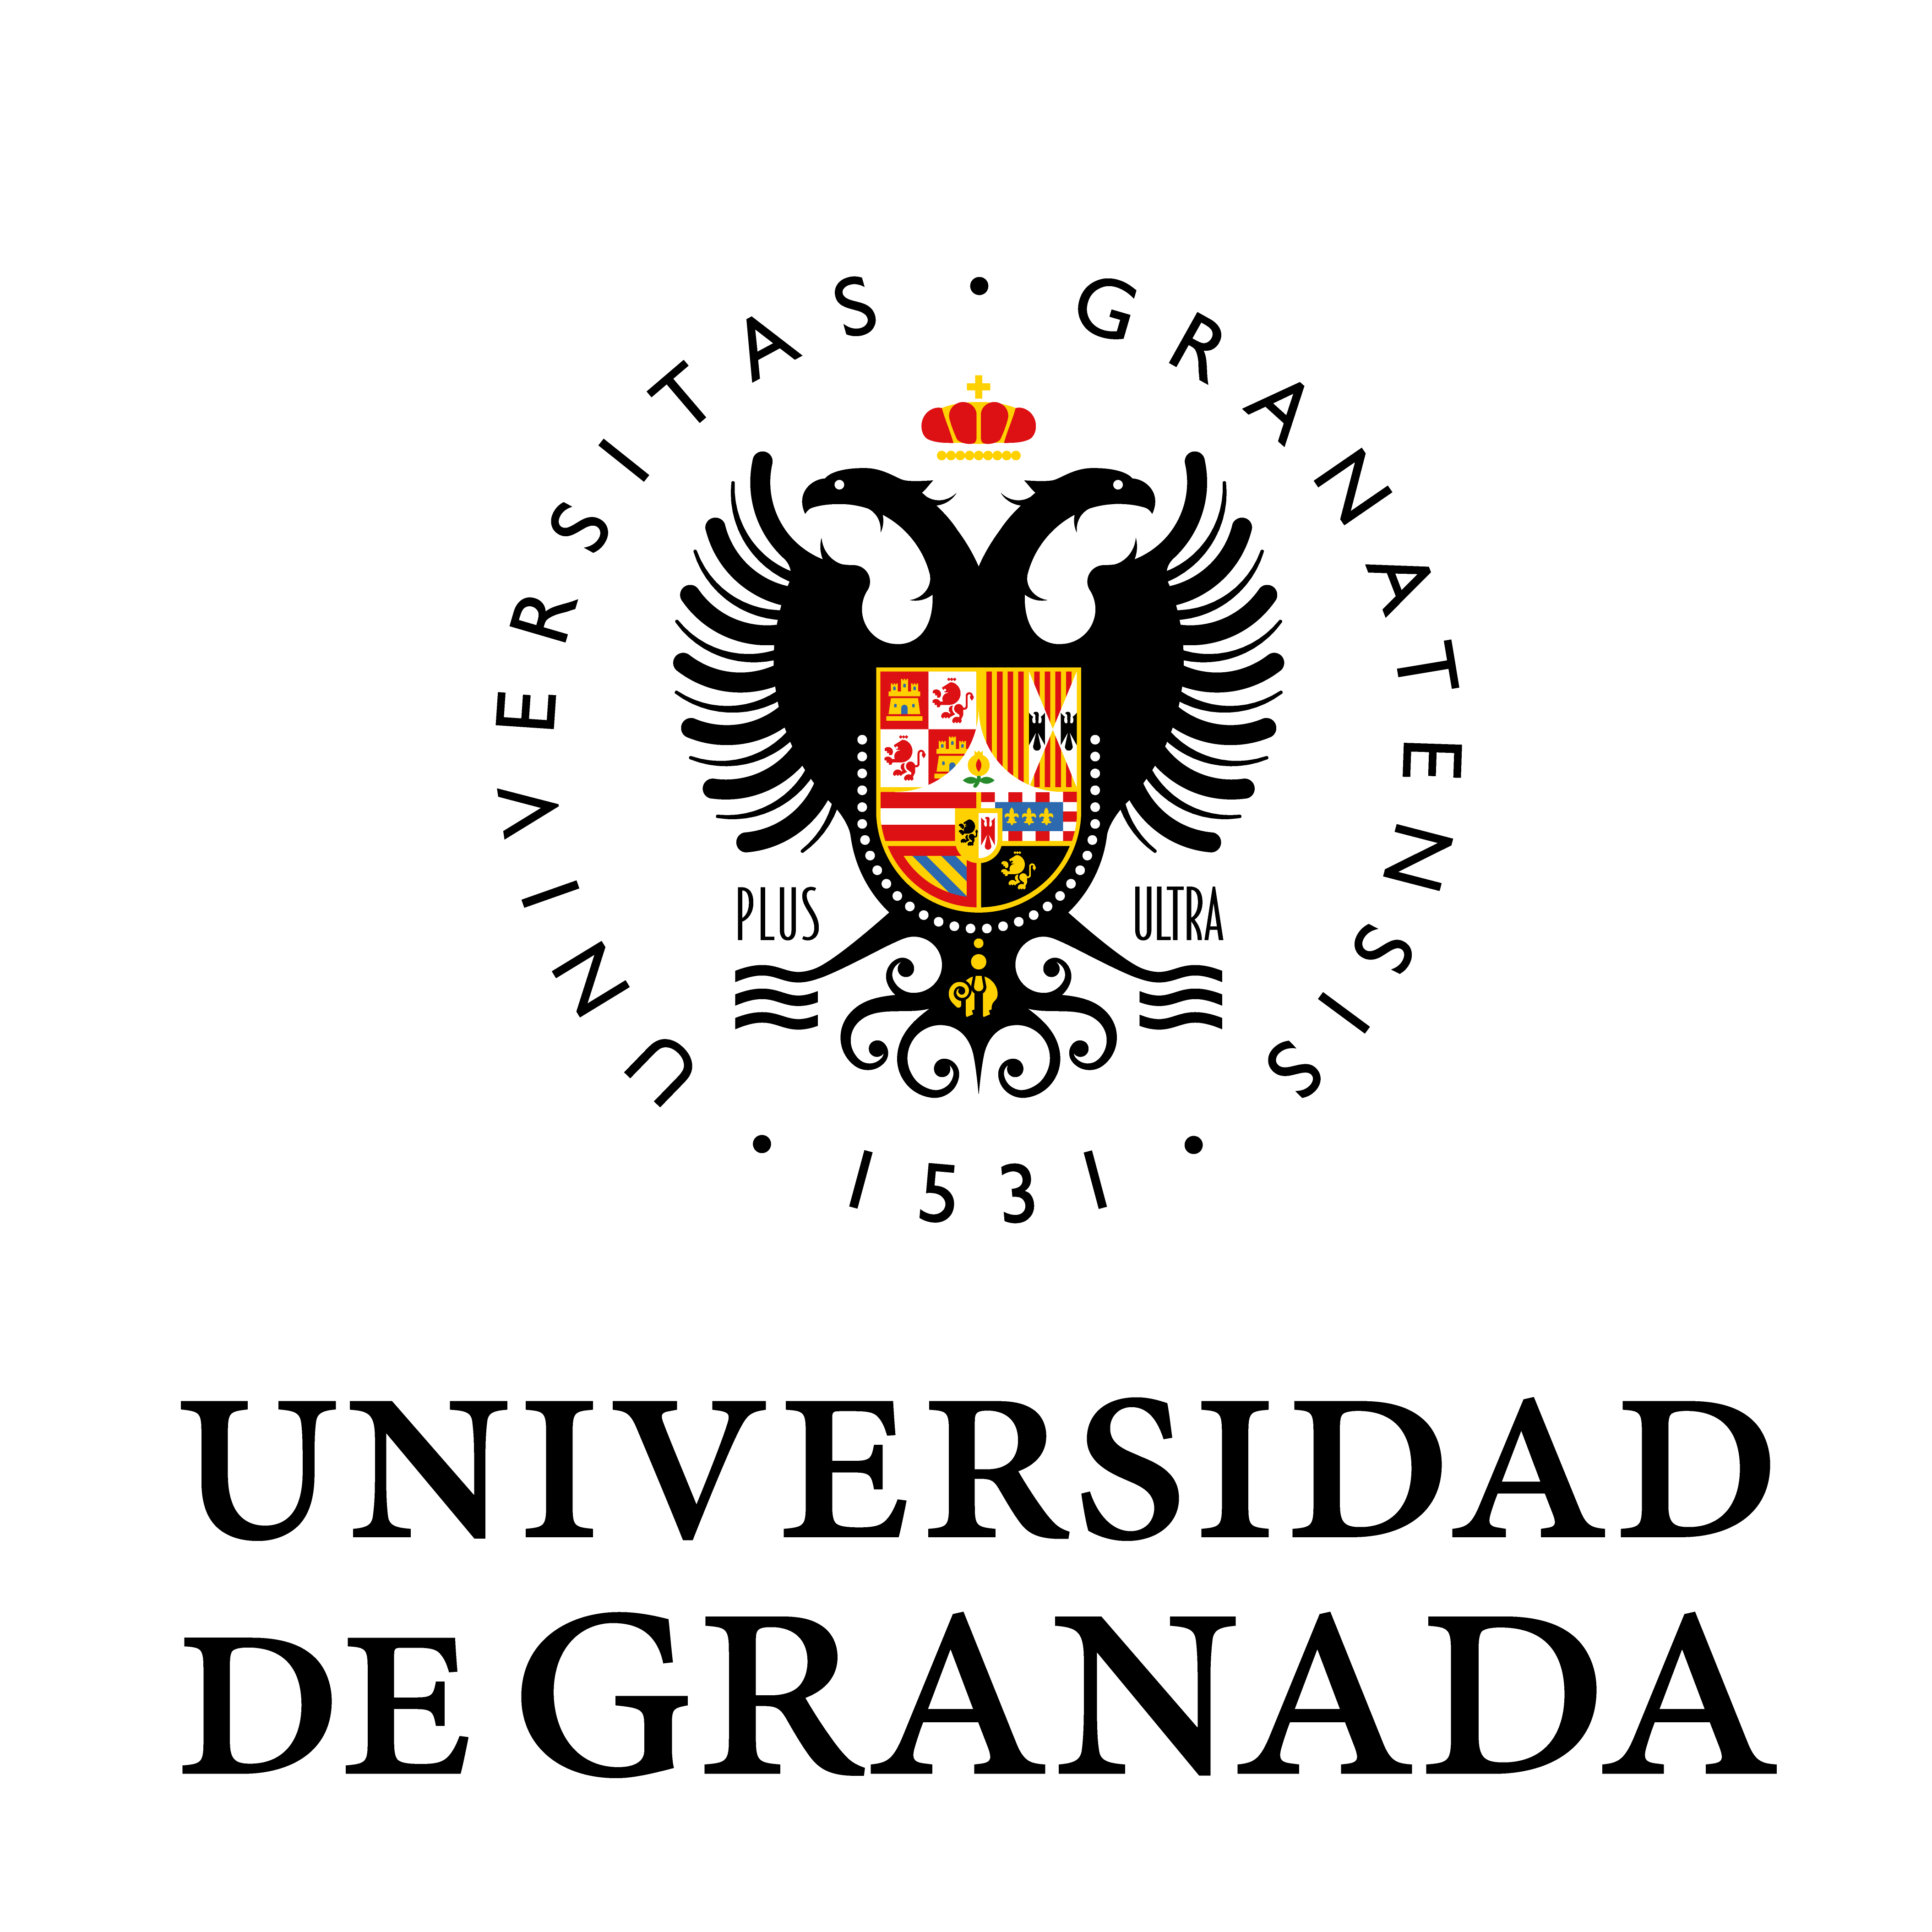
\includegraphics[width=0.9\textwidth]{./imagenes_memoria/ugr.png}\\[0.1cm]

\textsc{ \Large Práctica 2\\[0.1cm]}
\textsc{ \Large Ángel Cabeza Martín}\\
\textsc{ \Large 75571222F}\\
\textsl{ angelcabeza@correo.ugr.es}\\[0.3cm]
% Upper part of the page
% 
% Title
{\Huge\bfseries Detección de puntos relevantes y Construcción de panoramas\\
}
\noindent\rule[-1ex]{\textwidth}{2pt}\\[3.5ex]
{\large\bfseries Visión por Computador}
\end{titlepage}

%%%%%%%%%%%%%%%%%%%%%%%%%%%%%%%%%%%%%%%%%%%%%%%%%%%%%

\tableofcontents
\pagebreak
%%%%%%%%%%%%%%%%%%%%%%%%%%%%%%%%%%%%%%%%%%%%%%%%%%%%%

\section*{Introducción}
En esta práctica trabajaremos con la información de la geomtría de las imágenes, en concretro con la detección de puntos de interés, su detección y su uso para realizar otras operaciones como la detección de un objeto o zona de una imagen, que también nos permitirá crear panoramas de de imágenes. Trabajaremos con puntos de interés calculados (por nosotros) mediante SIFT y sus descriptores de puntos (estos calculados con OpenCV), y por último crearemos panoramas utilizando los puntos de interés y los descriptores calculados anteriormente\\


Por último, quiero aclarar que en esta memoria no me voy a centrar en explicar cómo he desarrollado mi código, si no en las decisiones que he tomado para desarrollar la práctica y los conceptos teóricos que me han guiado para tomar esas decisiones.


\section{Ejercicio 1: Extracción de regiones relevantes en un espacio de escalas}
Este ejercicio se centra en detectar puntos de interés (keypoints) construyendo un Espacio de Escalas de Lowe con cuatro octavas en total y tres escalas dentro de cada octava y el Espacio de Escalas Laplaciano para la detección de puntos de interés. Veremos durante los distintos apartados cómo he calculado el Espacio de Escalas y el Espacio de Escalas Laplaciano y todos los detalles de la implementación.

\subsection{¿Qué operaciones sobre la imagen original de $\sigma = 0.8$ nos permite fijar una imagen de semilla $\sigma = 1.6$}
Las operaciones que nos permiten fijar la semilla de 1.6 son upsampling de la imagen (aumentar el tamaño de la imagen al doble), la aplicación iterativa de los $\sigma$ calculados con la fórmula \ref{calculo_sigma_s} y por último downsampling (dividir el tamaño de la imagen a la mitad).

En esencia la idea es que convolucionar varias veces con un sigma pequeño es lo mismo que si suavizamos una única vez con un sigma grande,ya que la convolución de dos gaussianas es otra gaussiana y la convolución es asociativa. POr tanto suavizar dos veces con un kernel gaussiano de $\sigma$ es lo mismo que suavizar una vez con un kernel gaussiano de $\sigma * \sqrt[2]{2}$ y suavizar 3 veces con un kernel gaussiano de $\sigma$ es lo mismo que suavizar 3 veces con $\sqrt[2]{\sigma_1 + \sigma_2 + \sigma_3}$.

Por tanto para para ir de $\sigma = 0.5$ a $\sigma = 0.8$ habría que hacer $\sigma = \sqrt[2]{0.8² - 0.5²}$. Esto enlaza con SIFT porqu queremos obtener una imagen semilla con $\sigma = 1.6$ y nosotros empezamos con una imagen de 0.8, por lo tanto para hacer esto tendríamos que seguir los siguientes pasos:

\begin{itemize}
	\item Sigma inicial ($\sigma_0$) de captura igual a 0.8.
	\item Duplicamos el tamaño de la imagen y llegamos a v0.
	\item Aplicamos la fórmula \ref{calculo_sigma_s} y obtenemos los $\sigma$ hasta v3.
	\item Reducimos v3 y el resultado tendría que ser un $\sigma$ de 1.6.
\end{itemize}

Si lo hacemos así cada escala al principio de cada octava tiene $\sigma = 1.6$

\begin{figure}[H]
	\centering
	\[\sigma_s = \sigma_0 * \sqrt[2]{2^\frac{2s}{n_s} - 2^\frac{2(s-1)}{n_s}} \]
	\caption{Fórmula de  cálculo de $\sigma_s$.}
	\label{calculo_sigma_s}
\end{figure}

\subsection{Cálculo de escalas}
En este ejercicio se nos pide crear una función reusable que calcule las escalas de cualquier octava. Para ello he implementado la función \texttt{calculoescalas} que recibe como argumentos la imagen sobre la que calcular las escalas y el número de escalas que queremos obtener. La función realiza los siguientes pasos:


\begin{itemize}
	\item Añadimos la imagen pasada como argumento como la imagen inicial de la octava (la primera escala).
	\item Calculamos $\sigma_s$ con la fórmula \ref{calculo_sigma_s}.
	\item Calculamos el filtro gaussiano con $\sigma_s$.
	\item Convolucionamos la última escala calculada con la máscara calculada en el paso anterior.
	\item Añadimos la escala a la octava.
	\item Volver al segundo paso y repetir hasta llegar al número de escalas.
\end{itemize}

\subsection{Cálculo de octavas}
En este ejercicio se nos pide crear una función para calcular las escalas de todas las octavas. Para ello he creado la función \texttt{calcularoctavas} que recibe la imagen original sobre la que calcular la pirámide de Lowe y el número de octavas que se desean calcular. Para ello hago los siguientes pasos:

\begin{itemize}
	\item Primero upsampleaemos (duplicamos el tamaño de la imagen) la imagen para pasar de $\sigma = 0.8$ a $\sigma = 1.6$
	\item Llamamos a la función del ejercicio anterior para calcular la octava.
	\item Downsampleamos la imagen para que la primera imagen de la siguiente octava tenga $\sigma = 0.8$.
	\item Repetimos el paso 2 y 3 hasta tener tantas octavas como número octavas indique. 
\end{itemize}

Los downsampling y upsamplings los hacemos por lo que hemos comentado en el apartado 1. Tras aplicar esta función a las imágenes Yosemite1.jpg y Yosemite2.jpg hemos obtenido los siguientes resultados

\begin{figure}[H]
	\centering
	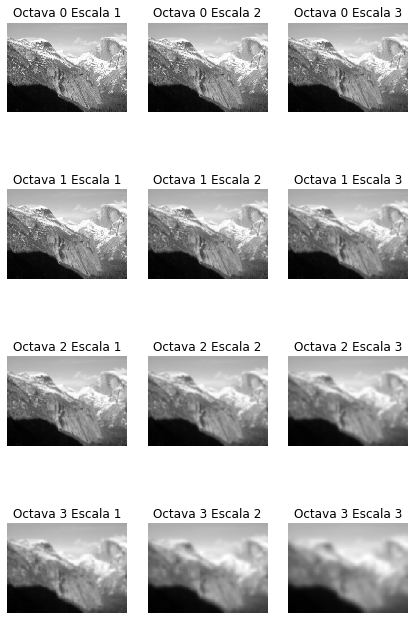
\includegraphics[width=12cm]{./imagenes_memoria/octavas_escalas.png}
	\caption{Pirámide de Lowe (solo 3 escalas por cada octava) de la imagen Yosemite1}
	\label{octavas_escalas}
\end{figure}

\begin{figure}[H]
	\centering
	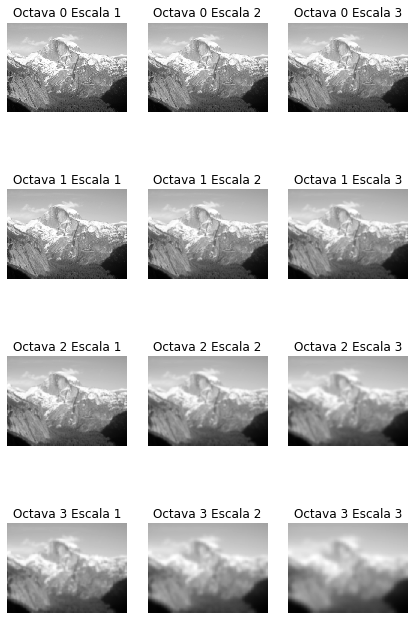
\includegraphics[width=12cm]{./imagenes_memoria/octavas_escalas2.png}
	\caption{Pirámide de Lowe (solo 3 escalas por cada octava) de la imagen Yosemite2}
	\label{octavas_escalas2}
\end{figure}

Como vemos estos resultados se ven aceptables porque conforme vamos aumentando la escala y la octava, las imágenes se ven mas borrosas puesto que estamos aplicando convoluciones iterativas.

\subsection{Cálculo de Espacio de Escalas Laplaciano e identificación de los 100 keypoints con más respuesta}
En este ejercicio se nos pide calcular el Espacio de Escalas Laplaciano y una vez obtenido identificar los keypoints y quedarnos con los 100 keypoints con más respuesta. Para calcular el Espacio de Escalas Laplaciano he creado la función \texttt{calcularEscalasDoG} que recibe una octava de la pirámide de Lowe y hace lo siguiente:

\begin{itemize}
	\item Para cada escala calcula la diferencia entre la escala actual y la escala anterior
	\item Esta diferencia será la nueva escala de la pirámide Laplaciana
\end{itemize}

y la función \texttt{calcularOctavasDoG} que como en la pirámide de Lowe calcula las octavas de la pirámide Laplaciana llamando a la función que hemos explicado anteriormente. Y así es como calculamos la pirámide Laplaciana.

Una vez calculada la pirámide Laplaciana podemos calcular los keypoints, para ello he creado la función \texttt{extraerKeypoints} que recibe la imagen inicial sobre la que extraer los keypoints, el número de octavas del Espacio de Escalas Laplaciano, el número de escalas, $\sigma_0$ (en nuestro caso 1.6) y el radio para posteriormente dibujarlos. Esta función realiza los siguientes pasos:

\begin{itemize}
	\item Calcular el Espacio de Escalas Laplaciano llamando a la función \texttt{calcularOctavasDoG}.
	\item Creo un array de keypoints donde guardo las coordenadas, la respuesta y la octava del punto
	\item Para cada octava del Espacio de Escalas Laplaciano:
		\begin{itemize}
			\item Creo una máscara de las dimensiones de la octava que nos servirá para no recorrer puntos dónde sabemos que no va a haber un extremo y de esta manera optimizar el cálculo de keypoints
			\item Para cada escala central:
				\begin{itemize}
					\item Recorremos la escala por columnas (saltándonos los bordes)
					\item Para cada fila (saltándonos los bordes):
						\begin{itemize}
							\item Miramos si el punto puede ser un keypoint (si la máscara tiene valor 0)
							\item Si es así miramos si es un extremo del vecindario (su vecindario son los puntos de alrededor de la escala actual, de la escala anterior y de la escala siguiente, estamos mirando en un espacio tridimensional):
							\item Si lo es calculamos $\sigma_k$ siguiendo la fórmula \ref{calculo_sigma_k} que nos servirá para almacenar el tamaño del círculo para luego poder dibujar los keypoints con un tamaño según su escala y modificamos la máscara para denotar los puntos que ya no pueden ser extremos			
						\end{itemize}							
				\end{itemize}
		\end{itemize}
	\item Devolver el array de keypoints.
\end{itemize}

\begin{figure}[H]
	\centering
	\[\sigma_k = \sigma_0 * 2^\frac{k}{n_s} \]
	\caption{Fórmula de  cálculo de $\sigma_k$.}
	\label{calculo_sigma_k}
\end{figure}

\subsection{Dibujar la imagen con los keypoints extraídos}
Con la función anterior obtenemos TODOS los keypoints de la imagen, ahora hay que ordenar el vector por el valor absoluto de la respuesta y despreciar los keypoints que no estén entre los 100 con más respuesta, una vez tenemos los 100 keypoints que nos interesan hay que convertirlos a keypoints de OpenCV mediante la función \texttt{KeyPoint} y por último hay que añadirlo a la imagen mediante la función \texttt{drawKeypoints} de OpenCV. Una vez hecho todo este proceso obtenemos los siguientes resultados:

\begin{figure}[H]
	\centering
	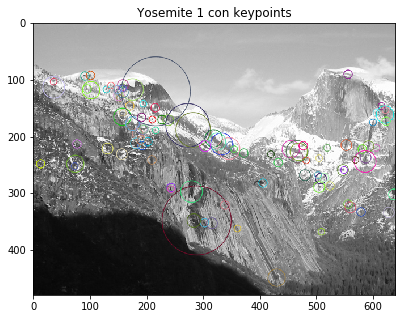
\includegraphics[width=12cm]{./imagenes_memoria/kpyose1.png}
	\caption{Yosemite1.jpg con sus 100 keypoints con mayor respuesta}
	\label{kp_yose1}
\end{figure}

\begin{figure}[H]
	\centering
	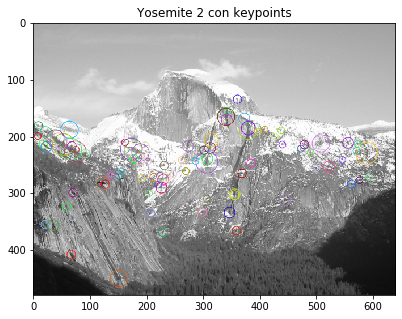
\includegraphics[width=12cm]{./imagenes_memoria/kpyose2.png}
	\caption{Yosemite2.jpg con sus 100 keypoints con mayor respuesta}
	\label{kp_yose2}
\end{figure}

Como podemos observar los keypoints tienen sentido porque están localizados en puntos de interés de la imagen (no hay ninguno en el cielo por ejemplo) y observamos que también hay keypoints detectados en escalas muy grandes. Pero siempre los keypoints van siguiendo la silueta de la figura, así como se ubican en zonas de importantes contrastes y texturas variadas. Me habría gustado comparar mis keypoints
con los que obtiene OpenCV pero no he tenido tiempo así que es algo que dejaré para el final del curso, pero la intuición dice que deberían salir distintos porque nosotros la implementación que hacemos de SIFT no es completa, pero las zonas por las que salen los keypoints tendrían que ser semejantes.


\section{Correspondencias}
En este apartado nos centraremos en detectar los puntos de interés así como sus descriptores utilizando la implementación de SIFT de OpenCV.

Para ello hemos utilizado el método \texttt{SIFTcreate} de OpenCV para obtener el detector SIFT con el que calcularemos los puntos clave y los descriptores de la imagen.

Para ello he usado el método \texttt{detectAndCompute} del detector que devuelve los keypoitns de la imagen y sus descriptores. \\

Una vez tenemos los descriptores y los keypoints de las dos imágenes tenemos que encontrar las correspondencias entre estas dos. Para eso usaremos dos métodos (ambos usan el objeto \texttt{BFMatcher} de OpenCV):

\begin{enumerate}
	\item Fuerza Bruta con validación cruzada.
	\item Clasificador 2NN aplicando el criterio de Lowe.
\end{enumerate}

Para el caso de fuerza bruta con validación cruzada he creado la función \texttt{FuerzaBruta} que recibe como parámetro las dos imágenes y el número de correspondencias a calcular, esta función sigue el siguiente proceso:

\begin{itemize}
	\item Crear el detector SIFT con la funcion \texttt{SIFTcreate} de OpenCV
	\item Calcular los puntos de interés y los descriptores de ambas imágenes con la funcion \texttt{detectAndCompute}
	\item Crear el matcher con la función \texttt{BFMatcher} con el parámetro crossCheck=True para hacer validación cruzada.
	\item Encontrar las correspondencias con la funcion \texttt{match} del matcher que hemos creado en el paso anterior.
	\item Dibujar 100 correspondencias aleatorias sobre las imágenes con la función \texttt{drawMatches} de OpenCV.
\end{itemize}

Para el caso de Lowe2NN he creado la función \texttt{coincidenciasLowe2NN} con los mismos parámetros que la función \texttt{FuerzaBruta}. Esta función hace exactamente lo mismo que la función anterior pero en lugar de utilizar el método \texttt{match} utilizaremos el método \texttt{knnMatch} con $k = 2$, y al resultado le aplicaremos el criterio de Lowe. Este criterio se basa en eliminar todas las coincidencias donde el radio de la distancia entre los puntos es mayor que $0.8$, consiguiendo eliminar alrededor de un 90\% de falsos positivos, y eliminando únicamente alrededor de un 5\% de coincidencias reales.

He obtenido los siguientes resultados:

\begin{figure}[H]
	\centering
	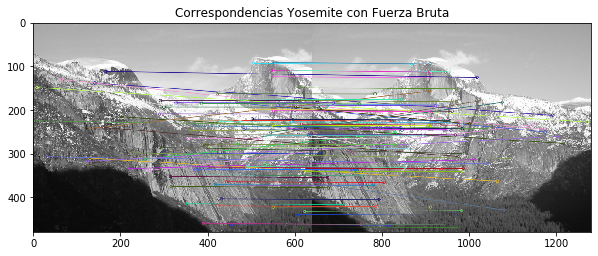
\includegraphics[width=12cm]{./imagenes_memoria/corrFB.png}
	\caption{Correspondencias de las imágenes Yosemite usando fuerza bruta}
	\label{kp_yose1}
\end{figure}

\begin{figure}[H]
	\centering
	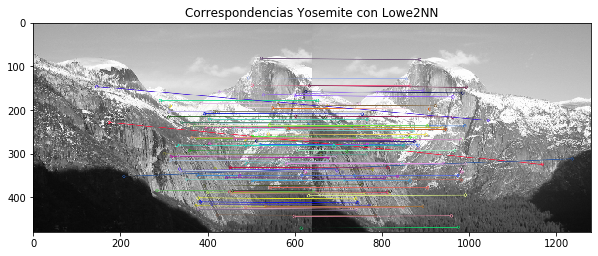
\includegraphics[width=12cm]{./imagenes_memoria/corrLW.png}
	\caption{Correspondencias de las imágenes Yosemite usando Lowe2NN}
	\label{kp_yose2}
\end{figure}

Como vemos, el método de fuerza bruta con validación cruzada es peor respecto al método de 2NN con el criterio de Lowe, ya que como podemos observar se consigue un número de errores considerablemente menor.

En especial vemos como la mayoría de fallos utilizando fuerza bruta se producen entre puntos con gran distancia, y en el caso en el que utilizamos el criterio de Lowe observamos que no se producen tantos errores y la distancia entre puntos se reduce.

\section{Construcción de un panorama rectangular}
En este ejercicio vamos a usar las correspondencias entre imágenes (trabajadas en el ejercicio anterior) para crear un panorama con tres imágenes.

En este caso, además de los puntos de interés y descriptores de una imagen también utilizaremos las homografías. Una homografía se trata de una relación entre dos imágenes que comparten el mismo plano, es decir, si dos imágenes son similares o iguales, pero tomadas desde distintas posiciones, ambas imágenes estarán relacionadas por una homografía, de forma que si aplicamos la homografía a una de estas obtendremos la otra. \\

Gracias a las homografías podemos conseguir crear un mosaico entre tres imágenes siguiendo los siguientes pasos:

\begin{enumerate}
	\item Elegir la imagen central de la lista de imágenes como centro
	\item Crear el canvas sobre el que ir añadiendo las imágenes.
	\item Construir la homografía que transforma la imagen elegida como centro al canvas ($H_0$) (ver cálculo \ref{H0})
	\item Calcular la homografía de la imagen situada a la izquierda de la central con la imagen central haciendo uso del método \texttt{findHomography} de OpenCV.
	\item Calcular la homografía de la imagen situada a la derecha de la central con la imagen central haciendo uso del método \texttt{findHomography} de OpenCV.
	\item Componer la homografía de la imagen de la izquierda a la imagen central con la homografía de traslación al canvas $H_0$ (para componer homografías simplemente se multiplican)
	\item Mover al canvas la imagen situada a la izquierda de la central usando la función \texttt{warpPerspective} de OpenCV y su homografía calculada en los pasos anterior.
	\item Componer la homografía de la imagen de la derecha a la imagen central con la homografía de traslación al canvas $H_0$ (para componer homografías simplemente se multiplican)
	\item Mover al canvas la imagen situada a la derecha de la central 
	usando la función \texttt{warpPerspective} de OpenCV y su homografía calculada en el pasos anterior.
	\item Finalmente mover al canvas la imagen central utilizando la homografía $H_0$
\end{enumerate}


\begin{figure}[H]
			\centering
			$\begin{pmatrix}
				1 & 0 & widthCanvas//2 - widthImagen1//2   \\
				0 & 1 & heightCanvas//2 - heightImagen1//2  \\
				0 & 0 & 1
			\end{pmatrix}$
			\caption{Cálculo de la homografía de traslación al canvas}
			\label{H0}
\end{figure}

Siguiendo estos pasos y recortando el canvas para eliminar las franjas negras para que se visualice mejor, he obtenido el siguiente resultado:

\begin{figure}[H]
	\centering
	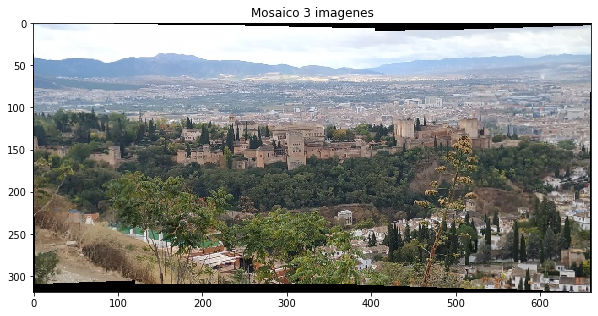
\includegraphics[width=12cm]{./imagenes_memoria/mosaico3.png}
	\caption{Mosaico Alhambra 3 imágenes}
	\label{mosaico3}
\end{figure}

Como vemos el resultado es bastante bueno y casi no se aprecia el cambio entre imágenes.

\subsection{Bonus B2 opción A: Construir un mosaico de N imágenes}
En este ejercicio se nos pide repetir el anterior ejercicio pero generalizando la función a N imágenes. Es por ello que la manera en la que vamos a calcular este mosaico no difiere en nada de la manera en la que calcular el mosaico de tres imágenes. \\

Para generalizarlo hay que crear el canvas y calcular todas las homografías (con \texttt{findHomography}) para pasar de una imágen a otra tal y como indica la siguiente figura \ref{calculo_homografias} en un ejemplo de 7 imágenes que es el que voy a utilizar para explicar cómo lo he hecho.

\begin{figure}[H]
	\centering
	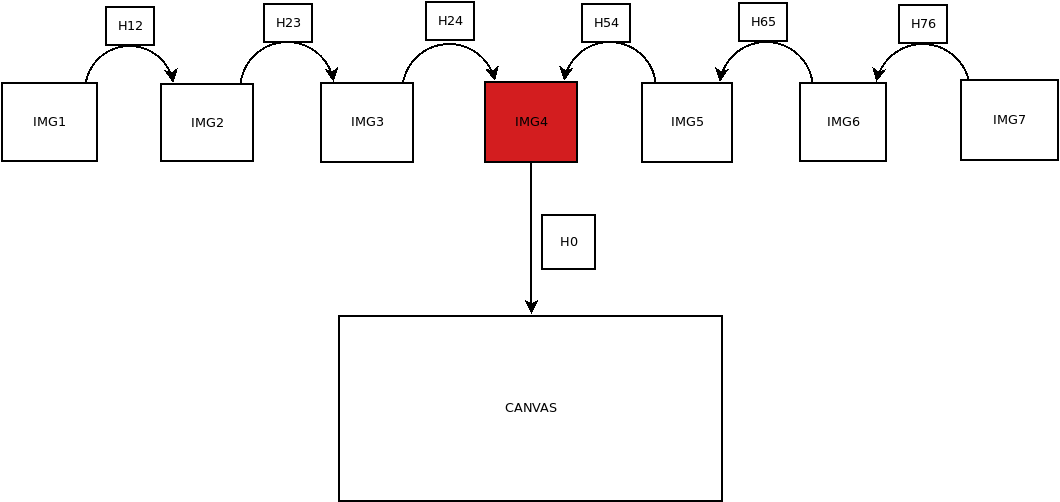
\includegraphics[width=12cm]{./imagenes_memoria/calchomo.png}
	\caption{Ejemplo cálculo homografías}
	\label{calculo_homografias}
\end{figure}

Una vez las tenemos calculadas hay que empezar a pasar las imágenes al canvas, para hacer esto hay que empezar desde un extremo (en mi caso he empezado en el extremo izquierda así que voy a explicarlo empezando desde ahí pero el orden da igual), por ejemplo la imágen en el extremo izquierda (IMG1 en la figura \ref{calculo_homografias_ej}). Para hacer esto hay que componer las distintas homografías de la siguiente forma (hay que hacer las operaciones de izquierda a derecha porque son operaciones matriciales):

\begin{figure}[H]
	\centering
	\[HT = H12 * H23 * H24 * H0 \]
	\caption{Ejemplo composición de homografías.}
	\label{calculo_homografias_ej}
\end{figure}

Y una vez calculado $HT$ mover la imagen al canvas usando la función \texttt{warpPerspective} y la homografía $HT$.

Una vez añadidas todas las imágenes hay que añadir la del centro tal y como lo hacíamos en el ejercicio anterior.

El resultado que obtengo es el siguiente: 

\begin{figure}[H]
	\centering
	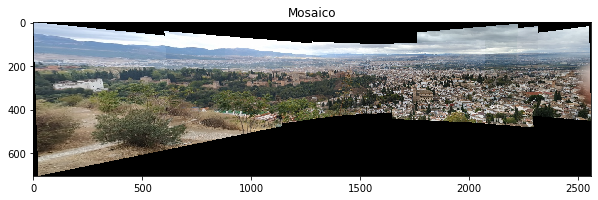
\includegraphics[width=12cm]{./imagenes_memoria/mosaicoN.png}
	\caption{Mosaico Alhambra N imágenes}
	\label{mosaicoN}
\end{figure}

\newpage

\section{Bibliografía}


\begin{thebibliography}{9}

	\bibitem{SIFT}

		Anatomy of the SIFT Method (Ives Rey-Otero, Mauricio Delbracio) Image Processing On Line, 2014

		\url{https://www.ipol.im/pub/art/2014/82/article.pdf}

	\bibitem{lowe}

		Distinctive Image Featuresfrom Scale-Invariant Keypoints (David G. Lowe)

		\url{https://www.cs.ubc.ca/~lowe/papers/ijcv04.pdf}

	\bibitem{keypoint}

		Clase KeyPoint - Documentación oficial de OpenCV

		\url{https://docs.opencv.org/master/d2/d29/classcv_1_1KeyPoint.html}

	\bibitem{drawKeypoints}

		drawKeypoints - Documentación oficial de OpenCV

		\url{https://docs.opencv.org/master/d4/d5d/group__features2d__draw.html#ga5d2bafe8c1c45289bc3403a40fb88920}


	\bibitem{detectCompute}

		detectAndCompute - Documentación oficial de OpenCV

		\url{https://docs.opencv.org/master/d0/d13/classcv_1_1Feature2D.html#a8be0d1c20b08eb867184b8d74c15a677}

	\bibitem{BFMatcher}

		Clase BFMatcher - Documentación oficial de OpenCV

		\url{https://docs.opencv.org/master/d3/da1/classcv_1_1BFMatcher.html}

	\bibitem{drawMatches}

		drawMatches - Documentación oficial de OpenCV

		\url{https://docs.opencv.org/master/d4/d5d/group__features2d__draw.html#gad8f463ccaf0dc6f61083abd8717c261a}

	\bibitem{knnMatch}

		knnMatch - Documentación oficial de OpenCV

		\url{https://docs.opencv.org/master/db/d39/classcv_1_1DescriptorMatcher.html#a378f35c9b1a5dfa4022839a45cdf0e89}

	\bibitem{match}

		match - Documentación oficial de OpenCV

		\url{https://docs.opencv.org/master/db/d39/classcv_1_1DescriptorMatcher.html#a0f046f47b68ec7074391e1e85c750cba}

	\bibitem{findHomography}

		findHomography - Documentación oficial de OpenCV

		\url{https://docs.opencv.org/master/d9/d0c/group__calib3d.html#ga4abc2ece9fab9398f2e560d53c8c9780}

	\bibitem{warpPerspective}

		warpPerspective - Documentación oficial de OpenCV

		\url{https://docs.opencv.org/master/da/d54/group__imgproc__transform.html#gaf73673a7e8e18ec6963e3774e6a94b87}

\end{thebibliography}

\end{document}

\end{document}
